\documentclass[convert=pdf2svg,multi=false]{standalone}
\usepackage{tikz}
  \usetikzlibrary{positioning}
\begin{document}
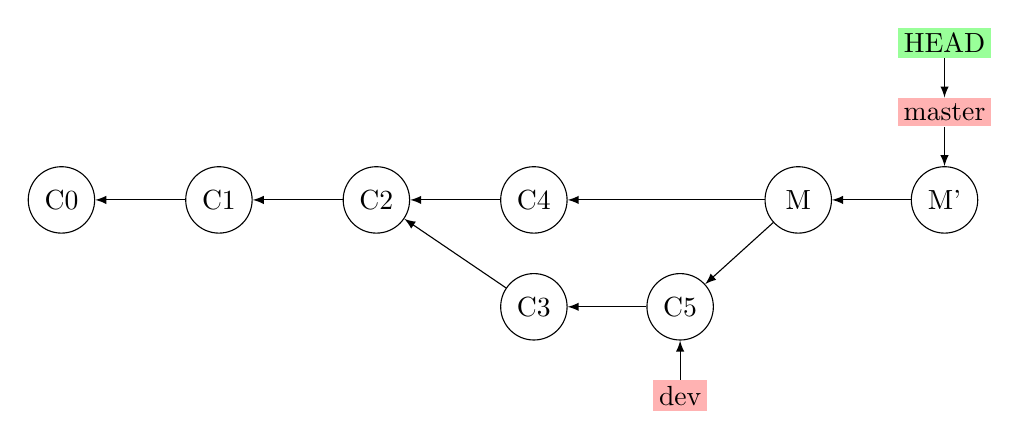
\begin{tikzpicture}[commit/.style={draw,circle,inner sep=2pt,minimum size=24pt},pointer/.style={draw=none,fill=red!30,rectangle,inner sep=2pt}]
\foreach \i[count=\x] in {0,1,2,4} {
   \node[commit] (C\i) at (2*\x,0) {C\i};
}
\node[commit, below=.5 of C4] (C3) {C3};
\node[commit, right=of C3] (C5) {C5};
\node[commit, right=2.5 of C4] (M) {M};
\node[commit, right=of M] (M') {M'};

\foreach \i/\j in {C0/C1,C1/C2,C2/C3,C2/C4,C3/C5,C4/M,C5/M,M/M'} {
  \draw[latex-] (\i) -- (\j);
}
% pointers
\node[pointer] (master) [above=.5 of M'] {master};
\node[pointer, fill=green!40] (head) [above=.5 of master] {HEAD};
\node[pointer] (dev) [below=.5 of C5] {dev};
\draw[-latex] (master) -- (M');
\draw[-latex] (head) -- (master);
\draw[-latex] (dev) -- (C5);
\end{tikzpicture}
\end{document}